\documentclass[noinstructornotes]{ximera}
%handout:  for handout version with no solutions or instructor notes
%handout,instructornotes:  for instructor version with just problems and notes, no solutions
%noinstructornotes:  shows only problem and solutions

%% handout
%% space
%% newpage
%% numbers
%% nooutcomes

%I added the commands here so that I would't have to keep looking them up
%\newcommand{\RR}{\mathbb R}
%\renewcommand{\d}{\,d}
%\newcommand{\dd}[2][]{\frac{d #1}{d #2}}
%\renewcommand{\l}{\ell}
%\newcommand{\ddx}{\frac{d}{dx}}
%\everymath{\displaystyle}
%\newcommand{\dfn}{\textbf}
%\newcommand{\eval}[1]{\bigg[ #1 \bigg]}

%\begin{image}
%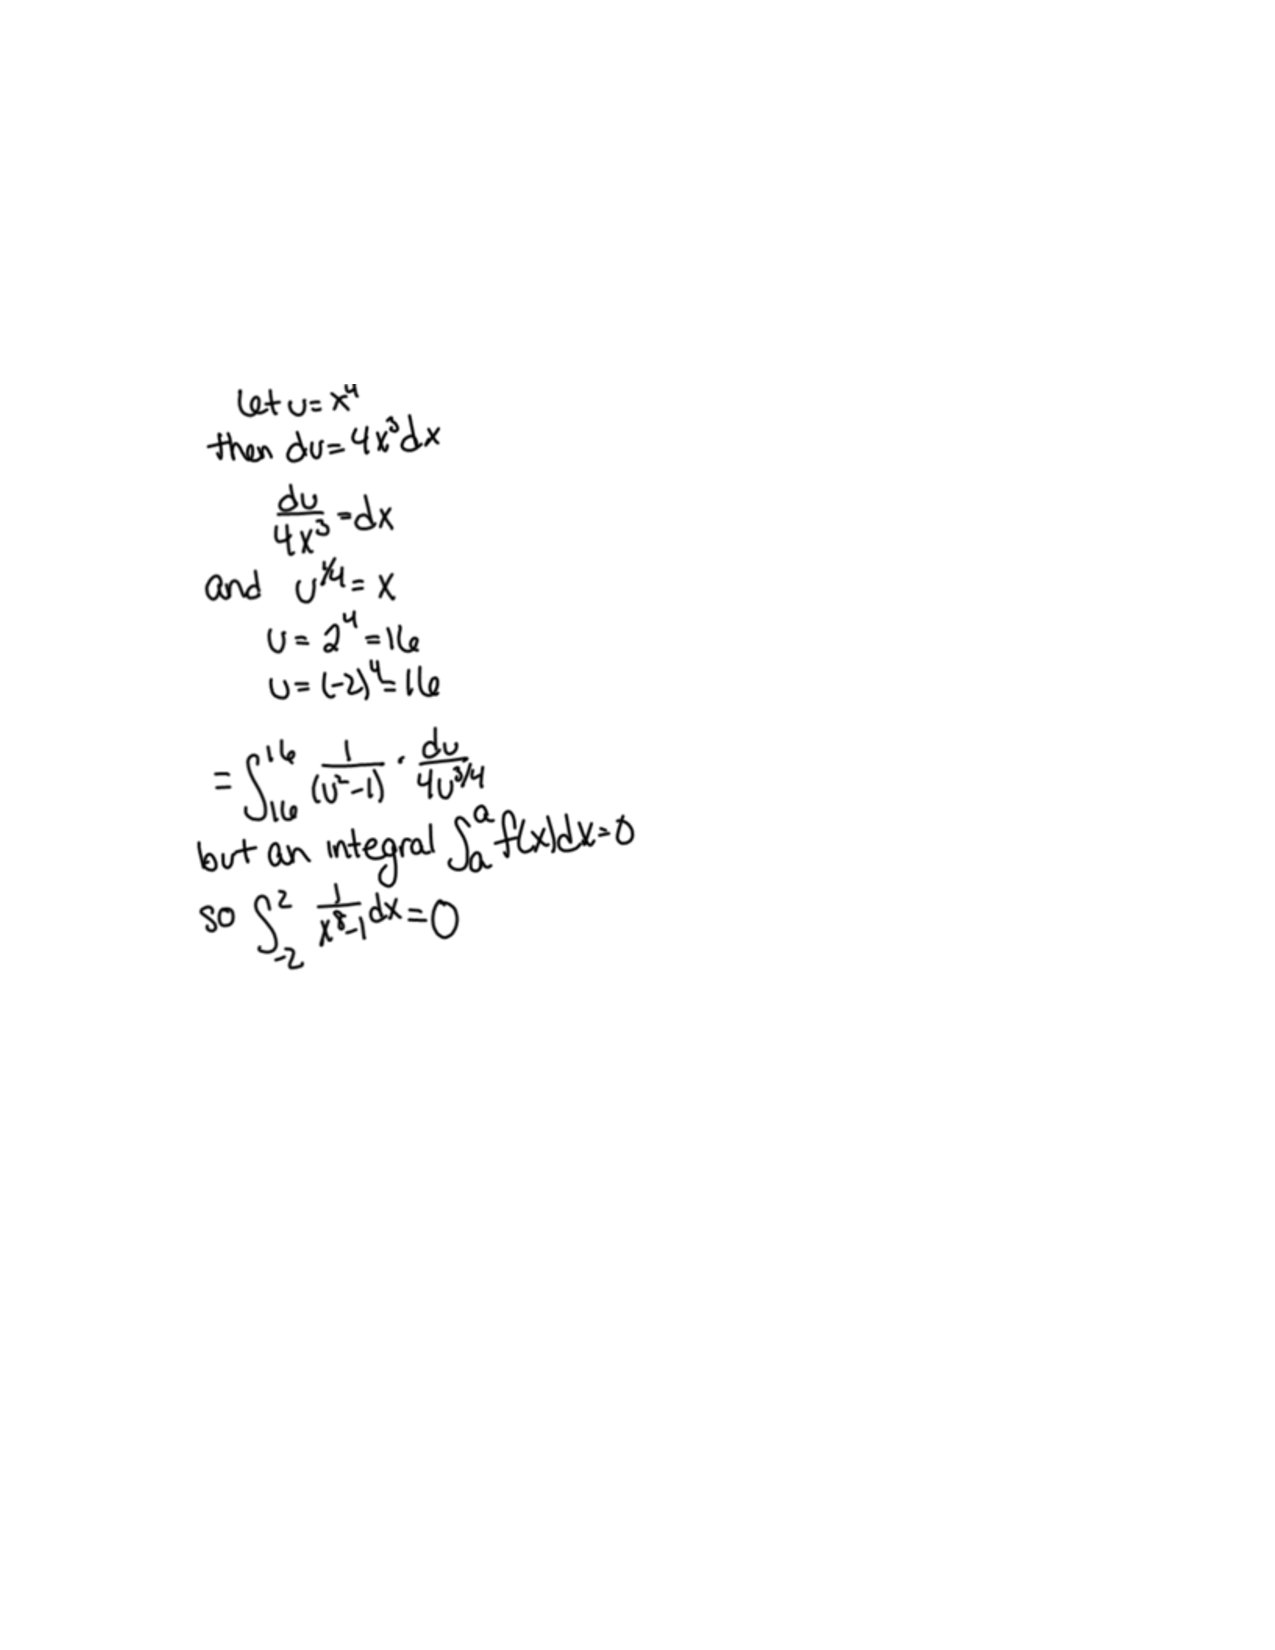
\includegraphics[trim= 170 420 250 180]{Figure1.pdf}
%\end{image}

%add a ``.'' below when used in a specific directory.
\newcommand{\RR}{\mathbb R}
\renewcommand{\d}{\,d}
\newcommand{\dd}[2][]{\frac{d #1}{d #2}}
\renewcommand{\l}{\ell}
\newcommand{\ddx}{\frac{d}{dx}}
\newcommand{\dfn}{\textbf}
\newcommand{\eval}[1]{\bigg[ #1 \bigg]}

\usepackage{multicol}

\renewenvironment{freeResponse}{
\ifhandout\setbox0\vbox\bgroup\else
\begin{trivlist}\item[\hskip \labelsep\bfseries Solution:\hspace{2ex}]
\fi}
{\ifhandout\egroup\else
\end{trivlist}
\fi} %% we can turn off input when making a master document


\title{Section 9.3: Infinite Series}  

\begin{document}
\begin{abstract}		\end{abstract}
\maketitle

\section{Warm-Up:}
\begin{problem}
Given a sequence $\{a_k\}_{k\geq1}$, explain how the sequence $\{s_k\}_{k\geq1}$of partial sums can be used to determine if the series $\displaystyle \sum_{k=1}^{\infty} a_k$ converges or diverges. 

\vspace{3mm}
\emph{Hint:} Recall that by definition $\displaystyle s_n = \sum_{k=1}^{n} a_k$
\end{problem}

\begin{freeResponse}
Note that $s_n = a_1+a_2+a_3+ \ldots + a_n$.  Thus, $s_n$ is a sequence whose $n^{th}$ term is the result of \emph{adding} the first $n$ terms in the sequence $\{a_k\}$.  If we continue adding the terms in the sequence $\{ a_k \}$ indefinitely, we will arrive at the infinite series $ \sum_{k=1}^{n} a_k$.  This result is obtained by taking the limit of the sequence $\{s_n\}$!  Formally, we can write: $$\lim_{n \rightarrow \infty} s_n = \sum_{k=1}^{\infty} a_k$$

Thus, we say $\displaystyle \sum_{k=1}^{\infty} a_k$ converges if and only if $\lim_{n \rightarrow \infty} s_n$ exists and $\displaystyle \sum_{k=1}^{\infty} a_k$ diverges if and only if $\lim_{n \rightarrow \infty} s_n$ does not exist.
\end{freeResponse}



\section{Group work:}










\begin{problem}
Determine if the following series converge or diverge.  If they converge, find the sum.
	\begin{enumerate}
	
	\item  $e + 1 + e^{-1} + e^{-2} + e^{-3} + \hdots$
	\begin{freeResponse}
		\begin{align*}
		e + 1 + e^{-1} + e^{-2} + e^{-3} + \hdots
		&= e + \sum_{k = 0}^\infty e^{-k}  \\
		&= e + \sum_{k=0}^\infty \left( e^{-1} \right)^k 	\quad	{\color{red}\text{geometric series, }r = e^{-1} < 1}  \\
		&= e + \frac{1}{1-e^{-1}}.
		\end{align*}
	Therefore, this series converges to $\left( e + \frac{1}{1-e^{-1}} \right)$.  
	\end{freeResponse}
	
	
	
	\item  $\sum_{k=0}^{99} 2^k + \sum_{k=100}^\infty \frac{1}{2^k}$
	\begin{freeResponse}
	Let us analyze the two different summands in this problem:
		\begin{enumerate}
		\item[(i)]  $\sum_{k=0}^{99} 2^k$
		
		This is a finite sum from a geometric sequence, and so its sum is 
			\[
			\frac{a(1-r^n)}{1-r}.
			\]
		Thus,
	  		\[
	  		\sum_{k=0}^{99} 2^k = \frac{1(1-2^{100})}{1-2} = 2^{100} - 1.
	  		\]
	  		
		\item[(ii)]  $\sum_{k=100}^\infty \frac{1}{2^k} = \sum_{k=100}^\infty \left( \frac{1}{2} \right)^k$.  
		
		This is a geometric series with $a=\frac{1}{2^{100}}$ and $r = \frac{1}{2}$.  
		So
			\[
			\sum_{k=100}^\infty \frac{1}{2^k} = \frac{\frac{1}{2^{100}}}{1-\frac{1}{2}} = \frac{1}{2^{99}}.
			\]
			
	Therefore, combining parts (i) and (ii) we have that
		\[
		\sum_{k=0}^{99} 2^k + \sum_{k=100}^\infty \frac{1}{2^k} = 2^{100} - 1 + \frac{1}{2^{99}}.
		\]
		\end{enumerate}
	\end{freeResponse}
	
	
	
	\item  $\sum_{k=0}^\infty (\cos(1))^k$
	\begin{freeResponse}
	This is a geometric series with $a=1$ and $r = \cos(1)$.  
	We know that $-1 < \cos(1) < 1$, and so $|\cos(1)|<1$.  
	Therefore, this geometric series converges and
		\begin{align*}
		\sum_{k=0}^\infty (\cos(1))^k = \frac{1}{1-\cos(1)}.
		\end{align*}
	\end{freeResponse}
	
	
	
	\item  $\sum_{k=4}^\infty \frac{5 \cdot 4^{k+3}}{7^{k-2}}$
	\begin{freeResponse}
	Let us first reindex this series.  
	Let $\ell = k-4$.  
	Then $k=\ell+4$, and when $k=4$, $\ell = 0$.
	We then have that
		\begin{align*}
		\sum_{k=4}^\infty \frac{5 \cdot 4^{k+3}}{7^{k-2}}
		&= \sum_{\ell=0}^\infty \frac{5 \cdot 4^{\ell + 4 + 3}}{7^{\ell + 4 - 2}}  \\
		&= \sum_{\ell=0}^\infty \frac{5 \cdot 4^{\ell + 7}}{7^{\ell + 2}}  \\
		&= \sum_{\ell=0}^\infty \frac{5 \cdot 4^7 \cdot 4^\ell}{7^2 \cdot 7^\ell}  \\
		&= \frac{5 \cdot 4^7}{7^2} \sum_{\ell=0}^\infty \left( \frac{4}{7} \right)^\ell  \quad	{\color{red}\text{assuming this series converges}}  \\
		&= \frac{5 \cdot 4^7}{7^2} \cdot \frac{1}{1-\frac{4}{7}}  \quad  {\color{red}\text{geometric series with }a=1, r = \frac{4}{7}}  \\
		&= \frac{5 \cdot 4^7}{3 \cdot 7}.
		\end{align*}
	Therefore, this series converges to $\frac{5 \cdot 4^7}{3 \cdot 7}$.  
	\end{freeResponse}
	
	
	
	\item  $\sum_{k=0}^\infty e^{5-2k}$
	\begin{freeResponse}
		\begin{align*}
		\sum_{k=0}^\infty e^{5-2k}
		&= \sum_{k=0}^\infty \left[ e^5 \cdot \left( e^{-2} \right)^k \right]  \\
		&= e^5 \sum_{k=0}^\infty \left( e^{-2} \right)^k  	\quad	{\color{red}\text{assuming the series converges}}  \\
		&= e^5 \cdot \frac{1}{1-e^{-2}}  \quad 	{\color{red}\text{geometric series with }a=1, r=e^{-2} < 1}
		\end{align*}
	Therefore, this series converges to $\frac{e^5}{1-e^{-2}}$.  
	\end{freeResponse}
	
	
	
%	\item  $\sum_{k=0}^\infty \frac{e^k + (-7)^k}{5^k}$
%	\begin{freeResponse}
%		\begin{align*}
%		\sum_{k=0}^\infty \frac{e^k + (-7)^k}{5^k} 
%		&= \sum_{k=0}^\infty \left[ \frac{e^k}{5^k} + \frac{(-7)^k}{5^k} \right]  \\
%		&= \sum_{k=0}^\infty \left[ \left( \frac{e}{5} \right)^k + \left( \frac{-7}{5} \right)^k \right] . \\
%		\end{align*}
%	If both of these series were convergent, then we would be able to split up the sum:
%		\[  
%		\sum_{k=0}^\infty \frac{e^k + (-7)^k}{5^k} ``=" \sum_{k=0}^\infty \left( \frac{e}{5} \right)^k + \sum_{k=0}^\infty \left( \frac{-7}{5} \right)^k.
%		\]
%	The first series on the right hand side is a geometric series with $r=\frac{e}{5}$.  
%	Since $\biggr| \frac{e}{5} \biggr| < 1$, this series converges.  
%	But the second series is a geometric series with $r = \frac{-7}{5}$.  
%	Since $\biggr| \frac{-7}{5} \biggr| > 1$, this series diverges.
%	
%	Therefore, the original series diverges.
%	\end{freeResponse}
%	
%	
%	
%	\item  $ \sum_{k=0}^\infty \left[ \frac{5}{(k+1)(k+2)} + \left( - \frac{1}{2} \right)^k \right]$
%	\begin{freeResponse}
%	If both series converge, then we can break up the sum:
%		\[
%		\sum_{k=0}^\infty \left[ \frac{5}{(k+1)(k+2)} + \left( - \frac{1}{2} \right)^k \right] = \sum_{k=0}^\infty \frac{5}{(k+1)(k+2)} + \sum_{k=0}^\infty \left( - \frac{1}{2} \right)^k.
%		\]
%	Let us consider both series on the right hand side of this equation individually.
%		\begin{enumerate}
%		\item[(i)]  $\sum_{k=0}^\infty \left( - \frac{1}{2} \right)^k$
%		
%		This is a geometric series with $a=1$ and $r = \frac{-1}{2}$.  
%		Therefore, this series converges with
%			\[
%			\sum_{k=0}^\infty \left( - \frac{1}{2} \right)^k = \frac{1}{1- \left( \frac{-1}{2} \right)}  = \frac{2}{3}.
%			\]
%		
%		\item[(ii)]  $\sum_{k=0}^\infty \frac{5}{(k+1)(k+2)}$
%		
%		It may not be obvious yet, but this is a telescoping series.  
%	To see this, let us decompose $\frac{5}{(k+1)(k+2)}$ as a partial fraction.
%		\begin{align*}
%		&\frac{5}{(k+1)(k+2)} = \frac{A}{k+1} + \frac{B}{k+2}  \\
%		\Longrightarrow 	\qquad 	&5 = A(k+2) + B(k+1).
%		\end{align*}
%	We solve for $A$ and $B$ by choosing ``smart" values for $k$:
%		\begin{align*}
%		&(k=-1) 	\quad	\Longrightarrow 	\quad	A = 5  \\
%		&(k=-2) 	\quad	\Longrightarrow		\quad	-B = 5 	\quad	\Longrightarrow		\quad	B = -5.
%		\end{align*}
%	So we see that
%		\begin{align*}
%		\sum_{i=1}^\infty \left( \frac{1}{i} - \frac{1}{i+2} \right) = \sum_{k=0}^\infty \left[ \frac{5}{k+1} - \frac{5}{k+2} \right].
%		\end{align*}
%	Let 
%		\[
%		S_n = \sum_{k=0}^n \left[ \frac{5}{k+1} - \frac{5}{k+2} \right].
%		\]
%	Then we have that
%		\begin{align*}
%		S_n &= \sum_{k=0}^n \left[ \frac{5}{k+1} - \frac{5}{k+2} \right]  \\
%		&= \left( \frac{5}{1} - \frac{5}{2} \right) + \left( \frac{5}{2} - \frac{5}{3} \right) + \left( \frac{5}{3} - \frac{5}{4} \right) + \hdots + \left( \frac{5}{n+1} - \frac{5}{n+2} \right)  \\
%		&= \frac{5}{1} - \frac{5}{n+2} = 5 - \frac{5}{n+2}.
%		\end{align*}
%	We then compute the sum by taking the limit of the sequence of partial sums:
%		\begin{align*}
%		\sum_{k=0}^\infty \frac{5}{(k+1)(k+2)}
%		&= \lim_{n \to \infty} \sum_{k=0}^n \frac{5}{(k+1)(k+2)}  \\
%		&= \lim_{n \to \infty} S_n  \\
%		&= \lim_{n \to \infty} \left( 5 - \frac{5}{n+2} \right)  \\
%		&= 5.
%		\end{align*}
%		\end{enumerate}
%	\vskip 5pt
%	Finally, we compute the sum of the original series as
%		\begin{align*}
%		\sum_{k=0}^\infty \left[ \frac{5}{(k+1)(k+2)} + \left( - \frac{1}{2} \right)^k \right] 
%		&= \sum_{k=0}^\infty \frac{5}{(k+1)(k+2)} + \sum_{k=0}^\infty \left( - \frac{1}{2} \right)^k  \\
%		&= 5 + \frac{2}{3} = \frac{17}{3}.
%		\end{align*}
%	\end{freeResponse}
%	
	
	
	\item  $\sum_{i=1}^\infty \left( \frac{2}{i^2+2i}  \right)$  
	Hint: $\frac{2}{i^2+2i} = \frac{1}{i} - \frac{1}{i+2}$ by partial fractions
	
	\begin{freeResponse}
	This is a telescoping series.  
	Let 
		\[
		S_n = \sum_{i=1}^n \left( \frac{1}{i} - \frac{1}{i+2} \right).
		\]
	Then,
		\begin{align*}
		S_n &= \sum_{i=1}^n \left( \frac{1}{i} - \frac{1}{i+2} \right)  \\
		&= \left( {\color{red}\frac{1}{1}} - \frac{1}{3} \right) + \left( {\color{red}\frac{1}{2}} - \frac{1}{4} \right) + \left( \frac{1}{3} - \frac{1}{5} \right) + \left( \frac{1}{4} - \frac{1}{6} \right) + \left( \frac{1}{5} - \frac{1}{7} \right)  \\
		&+ \hdots + \left( \frac{1}{n-2} - \frac{1}{n} \right) + \left( \frac{1}{n-1} - {\color{red}\frac{1}{n+1}} \right) + \left( \frac{1}{n} - {\color{red}\frac{1}{n+2}} \right)  \\
		&= 1 + \frac{1}{2} - \frac{1}{n+1} - \frac{1}{n+2}.
		\end{align*}
	Note that the last equality above is because all of the non-red terms cancel (convince yourself of this).  
	Then
		\begin{align*}
		\sum_{i=1}^\infty \left( \frac{1}{i} - \frac{1}{i+2} \right)
		&= \lim_{n \to \infty} S_n  \\
		&= \lim_{n \to \infty} \left[ 1 + \frac{1}{2} - \frac{1}{n+1} - \frac{1}{n+2} \right]  \\
		&= 1 + \frac{1}{2} = \frac{3}{2}.
		\end{align*}
	\end{freeResponse}
	
	\end{enumerate}
	
\end{problem}

\begin{instructorNotes}
Assign two per group.  
Most of these involve geometric series and one (part (b)) involves a finite geometric sum, whose ``trick'' is presented in the lecture.  

Students must identify the ``$r$'' and pay attention to both the indices and the exponents (for example, $7^{k+3} = 7^3 \cdot 7^k$).  
Encourage multiple methods (there are $3$ methods presented in the lecture) and make sure students clearly explain their reasoning on paper.  
\end{instructorNotes}







%%problem 2
%\begin{problem}
%Convert the decimal $2.456\overline{314}$ to a fraction using geometric series.
%	\begin{freeResponse}
%		\begin{align*}
%		2.456\overline{314}
%		&= 2.456 + 0.000314 + 0.000000314 + \hdots  \\
%		&= 2.456 + \frac{314}{1000^2} + \frac{314}{1000^3} + \hdots  \\
%		&= 2.456 + \sum_{k=1}^\infty \left[ \frac{314}{1000} \cdot \left( \frac{1}{1000} \right)^k \right]  \\
%		&= \frac{2456}{1000} + \frac{\frac{314}{1000^2}}{1 - \frac{1}{1000}}  \\
%		&=  \frac{2456}{1000} + \frac{\frac{314}{1000^2}}{\frac{999}{1000}}  \\
%		&= \frac{2456}{1000} + \frac{314}{999000}  \\
%		&= \frac{2453544 + 314}{999000}  \\
%		&= \frac{2453858}{999000} = \frac{1226929}{499500}.
%		\end{align*}
%	\end{freeResponse}
%
%\end{problem}
%
%\begin{instructorNotes}
%This is a common type of problem in this section.  
%Students have (most likely) never seen a problem with a non-repeating part to the decimal.  
%This should probably be done as a whole class.
%\end{instructorNotes}
%
%
%
%
%
%
%
%
%%problem 3
%\begin{problem}
%Find all values of $x$ for which the series 
%$$f(x) = \sum_{k=0}^\infty \frac{(x+3)^k}{2^k}$$ 
%converges.
%	\begin{freeResponse}
%	First notice that
%		\[
%		f(x) = \sum_{k=0}^\infty \frac{(x+3)^k}{2^k} = \sum_{k=0}^\infty \left( \frac{x+3}{2} \right)^k
%		\]
%	and so this is a geometric series with $a=1$ and $r = \frac{x+3}{2}$.  
%	So this series converges when
%		\begin{align*}
%		\biggr| &\frac{x+3}{2} \biggr| < 1  \\
%		\Longleftrightarrow 	\quad	-1 < &\frac{x+3}{2} < 1  \\
%		\Longleftrightarrow		\quad	-2 < &x+3 < 2  \\
%		\Longleftrightarrow		\quad	-5 < &x < -1.
%		\end{align*}
%	\end{freeResponse}
%		
%\end{problem}
%
%\begin{instructorNotes}
%The purpose of this problem is to give the students a preview of the idea of an interval of convergence (to be covered in Chapter 10).  
%Students need to be careful with absolute values and behavior at endpoints.  
%This could be skipped (or presented as a ``take home and think about it'' question).  
%\end{instructorNotes}










	
	
	
	
	
	
	
	
	

	










								
				
				
	














\end{document} 


















